\section{Atividade 3: Transformação e Representações Espaciais}
% Transformação e representação espacial (\textit{reshaping}), realizando a codificação das séries temporais 1D em representações matriciais 2D utilizando as técnicas de GAF e MTF.

As técnicas de codificação de séries temporais em representações matriciais bidimensionais, como o \textit{Gramian Angular Field} (GAF) e o \textit{Markov Transition Field} (MTF), são amplamente utilizadas em tarefas de mineração de dados, especialmente em problemas de classificação e agrupamento. Essas abordagens permitem capturar padrões temporais complexos que podem não ser evidentes em representações unidimensionais, então utilizamos a série de valores de retenção de valor (VRR) como base para a transformação em imagens. 

\subsection{Fundamentação}
% com base nos artigos de GAF e MTF descrever como que eh possivel transformar as imagens

A ideia central de \cite{wang2015imaging} é tratar uma série temporal como um sinal que pode ser reescrito em uma estrutura matricial, de modo que técnicas desenvolvidas para visão computacional passem a ser aplicáveis a dados temporais. O autor propõem três codificações: o \textit{Gramian Angular Summation Field} (GASF), o \textit{Gramian Angular Difference Field} (GADF) e o \textit{Markov Transition Field} (MTF). Esse tipo de abordagem também é adotado em trabalhos posteriores para agrupamento de séries, como em \cite{wu2023imaging}, que compara GASF, GADF, MTF e \textit{Recurrence Plots} (RP) e argumenta que a estrutura 2D reúne, em uma mesma representação, propriedades locais e relações de longo prazo da série.

\subsubsection{Gramian Angular Field (GASF e GADF)}

Dada uma série $X = \{x_1, x_2, \dots, x_n\}$, o primeiro passo é reescalonar seus valores para o intervalo $[0,1]$ (ou $[-1,1]$) por meio de uma normalização \textit{min-man}
\begin{equation}
\tilde{x}_i = \frac{x_i - \min(X)}{\max(X) - \min(X)}.
\label{eq:rescale}
\end{equation}
Em seguida, a série reescalonada é levada a coordenadas polares: o valor é codificado como o ângulo e o instante de tempo como o raio,
\begin{equation}
\begin{cases}
\phi_i = \arccos(\tilde{x}_i), & \tilde{x}_i \in \tilde{X},\\[2pt]
r_i = \dfrac{t_i}{N}, & t_i \in \mathbb{N},
\end{cases}
\label{eq:polar}
\end{equation}
em que $t_i$ é o carimbo de tempo e $N$ é uma constante que regulariza o intervalo do sistema polar. Como a função cosseno é monotônica em $[0,\pi]$, essa transformação é bijetora, isto é, cada série possui uma única representação polar e uma única inversa. Além disso, ao contrário das coordenadas cartesianas, a representação polar preserva as relações temporais absolutas \cite{wang2015imaging}.

Com os ângulos $\phi_i$, a correlação temporal entre os instantes $i$ e $j$ é obtida pela soma ou pela diferença trigonométrica dos ângulos:
\begin{align}
\mathrm{GASF} &= \left[\cos(\phi_i + \phi_j)\right] = \tilde{X}' \cdot \tilde{X} - \sqrt{I - \tilde{X}^2}' \cdot \sqrt{I - \tilde{X}^2}, \label{eq:gasf}\\
\mathrm{GADF} &= \left[\sin(\phi_i - \phi_j)\right] = \sqrt{I - \tilde{X}^2}' \cdot \tilde{X} - \tilde{X}' \cdot \sqrt{I - \tilde{X}^2}, \label{eq:gadf}
\end{align}
onde $I$ é o vetor linha unitário $[1,1,\dots,1]$. O resultado é uma matriz $n \times n$ (uma matriz de Gram quase-definida) na qual o tempo avança do canto superior esquerdo para o inferior direito. Assim, a dependência temporal é preservada, pois a entrada $(i,j)$ com $|i-j|=k$ representa a correlação relativa entre pontos separados por um intervalo $k$. A diagonal principal ($k=0$) contém a informação original do valor, de modo que, para dados reescalonados em $[0,1]$, é possível reconstruir a série a partir de $G_{ii} = \cos(2\phi_i)$ \cite{wang2015imaging}. Como a imagem tem tamanho $n \times n$, os autores sugerem o uso de \textit{Piecewise Aggregation Approximation} (PAA) para reduzir a resolução quando a série é longa.

\subsubsection{Markov Transition Field (MTF)}

Enquanto os campos angulares codificam informação estática (os valores e suas relações angulares), o MTF busca representar a dinâmica da série. A série é discretizada em $Q$ \textit{bins} de quantis e cada ponto $x_i$ recebe o \textit{bin} $q_j$ ao qual pertence ($j \in [1,Q]$). Contando as transições entre \textit{bins} consecutivos, à maneira de uma cadeia de Markov de primeira ordem, constrói-se a matriz de adjacência ponderada $W$ de tamanho $Q \times Q$, que, após normalização por linha ($\sum_j w_{ij}=1$), é a matriz de transição de Markov. Como $W$ é insensível à distribuição de $X$ e à dependência temporal, o MTF a espalha ao longo do eixo do tempo:
\begin{equation}
M = \begin{bmatrix}
w_{ij|x_1 \in q_i,\, x_1 \in q_j} & \cdots & w_{ij|x_1 \in q_i,\, x_n \in q_j}\\
\vdots & \ddots & \vdots\\
w_{ij|x_n \in q_i,\, x_1 \in q_j} & \cdots & w_{ij|x_n \in q_i,\, x_n \in q_j}
\end{bmatrix},
\label{eq:mtf}
\end{equation}
de forma que $M_{ij}$ é a probabilidade de transição entre o quantil do instante $t_i$ e o quantil do instante $t_j$. A diagonal principal $M_{ii}$ corresponde à probabilidade de autotransição naquele instante \cite{wang2015imaging}. Assim, o GAF e o MTF fornecem visões complementares da mesma série, e \cite{wang2015imaging} propõem tratá-las como canais ``ortogonais'' (como as cores de uma imagem RGB), empilhando GASF, GADF e MTF em uma imagem de três canais. O MTF, porém, possui um espaço de imagens inversas muito maior que o do GAF, o que dificulta recuperar o sinal original e explica, segundo os autores, seu desempenho isolado geralmente inferior ao dos campos angulares na classificação. Por fim, \cite{wu2023imaging} indicam que as quatro codificações têm custo computacional $O(n^2)$ e que a escolha do método de imageamento influencia de forma relevante o resultado de tarefas de agrupamento.

\subsection{Metodologia}
% descrever como foi feita a transformação (mapeando os dados seriados de depreciação), as janelas escolhidas e o output final (imagens e arquivos)

O fluxo do trabalho inicia com a série de entrada sendo a taxa de retenção de valor (VRR) de cada veículo, que é codificada em imagens GASF, GADF e MTF. Para cada janela de tamanho $T \in \{24, 32, 48, 64\}$ meses, são selecionados veículos lançados a partir de 2019 que possuem histórico completo para os primeiros $T$ meses. Meses ausentes são preenchidos por interpolação linear, e séries com mais de $10\%$ de meses ausentes são descartadas. Cada série é reescalonada globalmente em $[0,1]$, e o MTF é calculado com $Q=8$ \textit{bins} de quantis por série. As saídas incluem as imagens codificadas, as séries brutas de VRR e metadados dos veículos. A Figura \ref{fig:pipeline_encoding} ilustra o processo completo dessa geração.

\begin{figure}[!hbtp]
    \centering
    \resizebox{0.85\columnwidth}{!}{%
    \begin{tikzpicture}[
        % Estilos (mesmos do pipeline1.tex)
        recntagle/.style={
            rectangle, rounded corners=3pt, inner sep=6pt, align=center,
            font=\small\bfseries, draw=black!70, fill=blue!10, line width=0.8pt
        },
        title_block/.style={
            rectangle, rounded corners=3pt, inner sep=4.5pt, align=center,
            font=\small\bfseries, draw=black!70, fill=blue!10, line width=0.8pt
        },
        arrow/.style = {
            thick, ->, >={Stealth[length=2.5mm]}
        },
        box_delimitador/.style = {
            rectangle, rounded corners=8pt, draw=black!70, fill=black!2, line width=0.8pt
        },
        sub_block/.style = {
            rectangle, rounded corners=3pt, inner sep=6pt, align=center,
            draw=black!70, fill=blue!5, line width=0.7pt, font=\small
        },
        embed_block/.style = {
            rectangle, rounded corners=3pt, inner sep=6pt, align=center,
            draw=black!70, fill=blue!15, line width=0.7pt, font=\small\bfseries
        },
        file_block/.style = {
            rectangle, rounded corners=3pt, inner sep=5pt, align=center,
            draw=black!70, fill=white, line width=0.7pt, font=\footnotesize
        }
    ]

        % 1. Entrada de dados
        \node (input) [recntagle, minimum width=5cm] {1. Dados FIPE (\texttt{.parquet})};

        % 2. PRÉ-PROCESSAMENTO
        \node (pre_box) [box_delimitador, minimum width=13cm, minimum height=2.8cm, below=0.8cm of input] {};
        \node (pre_title) [title_block] at (pre_box.north) {2. Pré-processamento};

        \node (clean) [sub_block, text width=5.2cm] at ([xshift=-3.4cm, yshift=-0.35cm]pre_box.center) {Limpeza e filtros\\(duplicados, valor zero,\\carros, marcas relevantes)};
        \node (vrr) [sub_block, text width=5.2cm] at ([xshift=3.4cm, yshift=-0.35cm]pre_box.center) {Taxa de Retenção de Valor (VRR)\\ancorada no mês zero\\($\mathrm{VRR}_t = \mathrm{valor}_t / \mathrm{valor}_0$)};

        \draw [arrow] (input.south) -- (pre_title.north);
        \draw [arrow] (clean.east) -- (vrr.west);

        % 3. CONSTRUÇÃO DAS SÉRIES
        \node (series_box) [box_delimitador, minimum width=13cm, minimum height=3.0cm, below=0.8cm of pre_box] {};
        \node (series_title) [title_block] at (series_box.north) {3. Construção das Séries};

        \node (window) [sub_block, text width=3.5cm] at ([xshift=-4.4cm, yshift=-0.35cm]series_box.center) {Janelas\\$T \in \{24, 32, 48, 64\}$ meses\\(lançamento $\geq$ 2019)};
        \node (interp) [sub_block, text width=3.5cm] at ([xshift=0cm, yshift=-0.35cm]series_box.center) {Interpolação linear\\(descarta séries com\\$>$ 10\% de meses faltantes)};
        \node (scale) [sub_block, text width=3.5cm] at ([xshift=4.4cm, yshift=-0.35cm]series_box.center) {Escala global\\$\mathrm{VRR}/1{,}5$ em $[0,1]$\\(com \textit{clipping})};

        \draw [arrow] (pre_box.south) -- (series_title.north);
        \draw [arrow] (window.east) -- (interp.west);
        \draw [arrow] (interp.east) -- (scale.west);

        % 4. CODIFICAÇÃO EM IMAGENS
        \node (enc_box) [box_delimitador, minimum width=13cm, minimum height=3.2cm, below=0.8cm of series_box] {};
        \node (enc_title) [title_block] at (enc_box.north) {4. Codificação 2D ($T \times T$, sem PAA)};

        \node (gasf) [embed_block, text width=3.5cm] at ([xshift=-4.4cm, yshift=-0.35cm]enc_box.center) {GASF\\{\footnotesize\mdseries $\cos(\phi_i + \phi_j)$}};
        \node (gadf) [embed_block, text width=3.5cm] at ([xshift=0cm, yshift=-0.35cm]enc_box.center) {GADF\\{\footnotesize\mdseries $\sin(\phi_i - \phi_j)$}};
        \node (mtf) [embed_block, text width=3.5cm] at ([xshift=4.4cm, yshift=-0.35cm]enc_box.center) {MTF\\{\footnotesize\mdseries 8 \textit{bins} de quantis}};

        \draw [arrow] (series_box.south) -- (enc_title.north);

        % 5. SAÍDAS
        \node (out_box) [box_delimitador, minimum width=13cm, minimum height=3.2cm, below=0.8cm of enc_box] {};
        \node (out_title) [title_block] at (out_box.north) {5. Saídas por Janela (\texttt{window\_TT/})};

        \node (f_img) [file_block, text width=2.6cm] at ([xshift=-4.65cm, yshift=-0.35cm]out_box.center) {\texttt{gasf.npy}\\\texttt{gadf.npy}\\\texttt{mtf.npy}\\$(N, T, T)$};
        \node (f_ser) [file_block, text width=2.6cm] at ([xshift=-1.55cm, yshift=-0.35cm]out_box.center) {\texttt{series\_vrr.npy}\\$(N, T)$\\(bases Euclidiana/DTW)};
        \node (f_meta) [file_block, text width=2.6cm] at ([xshift=1.55cm, yshift=-0.35cm]out_box.center) {\texttt{metadata.parquet}\\+ segmento de preço\\(Entrada / Interm. / Luxo)};
        \node (f_cfg) [file_block, text width=2.6cm] at ([xshift=4.65cm, yshift=-0.35cm]out_box.center) {\texttt{config.json}\\\texttt{examples\_*.png}};

        \draw [arrow] (enc_box.south) -- (out_title.north);

    \end{tikzpicture}%
    }
    \caption{Fluxo da metodologia de codificação das séries de retenção de valor (VRR) em imagens GASF, GADF e MTF.}
    \label{fig:pipeline_encoding}
\end{figure}


\subsubsection{Série de entrada: taxa de retenção de valor}

A série a ser codificada é a \textit{Value Retention Rate} (VRR) de cada veículo. Após a limpeza e o pré-processamento dos dados da tabela FIPE (remoção de registros duplicados e de valor zero, filtro para carros, exclusão de combustíveis gás natural e etanol, filtro de marcas relevantes e de veículos lançados há mais de 20 anos), cada coorte é identificada pela chave (\texttt{codigo\_fipe}, \texttt{ano\_modelo}, \texttt{sigla\_combustivel}). A idade do veículo em meses (\texttt{idade\_meses}) é calculada como a diferença entre o mês de referência e o mês da primeira cotação (\texttt{data\_lancamento}), e a VRR é definida como
\begin{equation}
\mathrm{VRR}_t = \frac{\text{valor}_t}{\text{valor}_{t=0}},
\end{equation}
em que o preço de lançamento $\text{valor}_{t=0}$ é ancorado na cotação do mês zero (\texttt{idade\_meses} $=0$). Dessa forma, toda série começa em $100\%$ e descreve a evolução relativa do valor do veículo, independentemente do seu preço absoluto.

\subsubsection{Janelas e seleção de veículos}

Foram definidas quatro janelas, $T \in \{24, 32, 48, 64\}$ meses. Para cada janela, entram na amostra os veículos lançados a partir de 2019 que possuem histórico cobrindo os meses $0$ a $T-1$, e cada veículo é representado pelos seus primeiros $T$ meses de VRR. Quando há mais de um registro para o mesmo veículo e mês, utiliza-se a média. Meses ausentes dentro da janela são preenchidos por interpolação linear, e séries cuja fração de meses ausentes excede $10\%$ da janela são descartadas. A quantidade de veículos varia de acordo com a janela, já que janelas maiores exigem históricos mais longos.

\subsubsection{Codificação em imagens}

Cada série é codificada em três imagens $T \times T$, sem PAA e sem redimensionamento (ou seja, o tamanho da imagem é $S=T$), de modo a preservar toda a resolução temporal. As adaptações em relação ao procedimento original de \cite{wang2015imaging} são as seguintes:
\begin{itemize}
    \item \textbf{Reescalonamento global em $[0,1]$.} Em vez do \textit{min-max} por série da Equação~\ref{eq:rescale}, utiliza-se uma escala fixa e comum a todos os veículos, $\tilde{x} = \mathrm{VRR}/1{,}5$, com recorte (\textit{clipping}) em $[0,1]$ (o valor máximo de VRR é fixado em $150\%$). Com isso, o nível absoluto de depreciação (ou valorização) é preservado entre veículos diferentes, o que não ocorreria com a normalização individual. A fração de valores recortados é registrada para cada janela. O intervalo $[0,1]$ é o mesmo para o qual \cite{wang2015imaging} demonstram a bijetividade do GASF.
    \item \textbf{GASF e GADF.} Calculados conforme as Equações~\ref{eq:gasf} e \ref{eq:gadf}, de forma vetorizada para todos os veículos, em precisão \texttt{float32}.
    \item \textbf{MTF.} Calculado com $Q=8$ \textit{bins} e estratégia de quantis por série, como no artigo original, de modo que cada série é discretizada pelos seus próprios quantis. A matriz $W$ é estimada pelas transições consecutivas e normalizada por linha, e o campo é obtido por $M_{ij} = W[\mathrm{bin}(x_i), \mathrm{bin}(x_j)]$ (Equação~\ref{eq:mtf}). Como os quantis são relativos a cada série, o MTF descreve a dinâmica, mas não o nível absoluto da VRR; esse nível é preservado pelos campos angulares. A implementação também aceita \textit{bins} uniformes sobre a escala global, o que manteria a informação de nível.
\end{itemize}

\subsubsection{Segmentação por faixa de preço}

Para analisar o comportamento de cada tipo de veículo, os veículos foram segmentados pelo preço de lançamento, a partir do primeiro (Q1) e do terceiro quartil (Q3) dos preços de todos os veículos únicos lançados desde 2019, independentemente do tamanho do histórico (mesmo procedimento da análise exploratória): \textbf{Entrada} (preço $\le$ Q1), \textbf{Intermediário} (Q1 $<$ preço $\le$ Q3) e \textbf{Luxo} (preço $>$ Q3).

\subsubsection{Saídas geradas}

Para cada janela $T$ é criada uma pasta \texttt{window\_TT} com os arquivos listados na Tabela~\ref{tab:saidas}, todos com a mesma ordem de veículos.

% Certifique-se de incluir no preâmbulo: \usepackage{tabularx} e \usepackage{booktabs}

\begin{table}[htbp]
\centering
\caption{Arquivos gerados para cada janela de $T$ meses ($N$ é o número de veículos da janela).}
\label{tab:saidas}
\begin{tabularx}{\columnwidth}{@{} l X @{}}
\toprule
\textbf{Arquivo} & \textbf{Conteúdo} \\
\midrule
\texttt{gasf.npy}, \texttt{gadf.npy}, \texttt{mtf.npy} & Imagens \texttt{float32} de dimensão $(N, T, T)$ \\ \addlinespace
\texttt{series\_vrr.npy} & Séries VRR brutas $(N, T)$, em razão, para as bases Euclidiana/DTW \\ \addlinespace
\texttt{metadata.parquet} & Uma linha por veículo (modelo, marca, combustível, preço de lançamento, segmento etc.) \\ \addlinespace
\texttt{config.json} & Parâmetros usados (janela, escala, \textit{bins}, \textit{clipping}, Q1 e Q3) \\ \addlinespace
\texttt{examples\_fuel.png}, \texttt{examples\_segments.png} & Exemplos por combustível e por faixa de preço \\
\bottomrule
\end{tabularx}
\end{table}

\subsection{Resultados}
% dar include graphics de cada uma das janelas usando 'examples_segments.png' que tem os exemplos separados pelas faixas de valores

As Figuras~\ref{fig:w24} a \ref{fig:w64} mostram, para cada janela, um veículo sorteado aleatoriamente (semente fixa) de cada faixa de preço, com a série de VRR (em \%) e as respectivas imagens GASF, GADF e MTF. Como os veículos sorteados diferem entre as janelas, as figuras ilustram o comportamento das codificações e não permitem comparar um mesmo veículo entre janelas.

\begin{figure}[htbp]
    \centering
    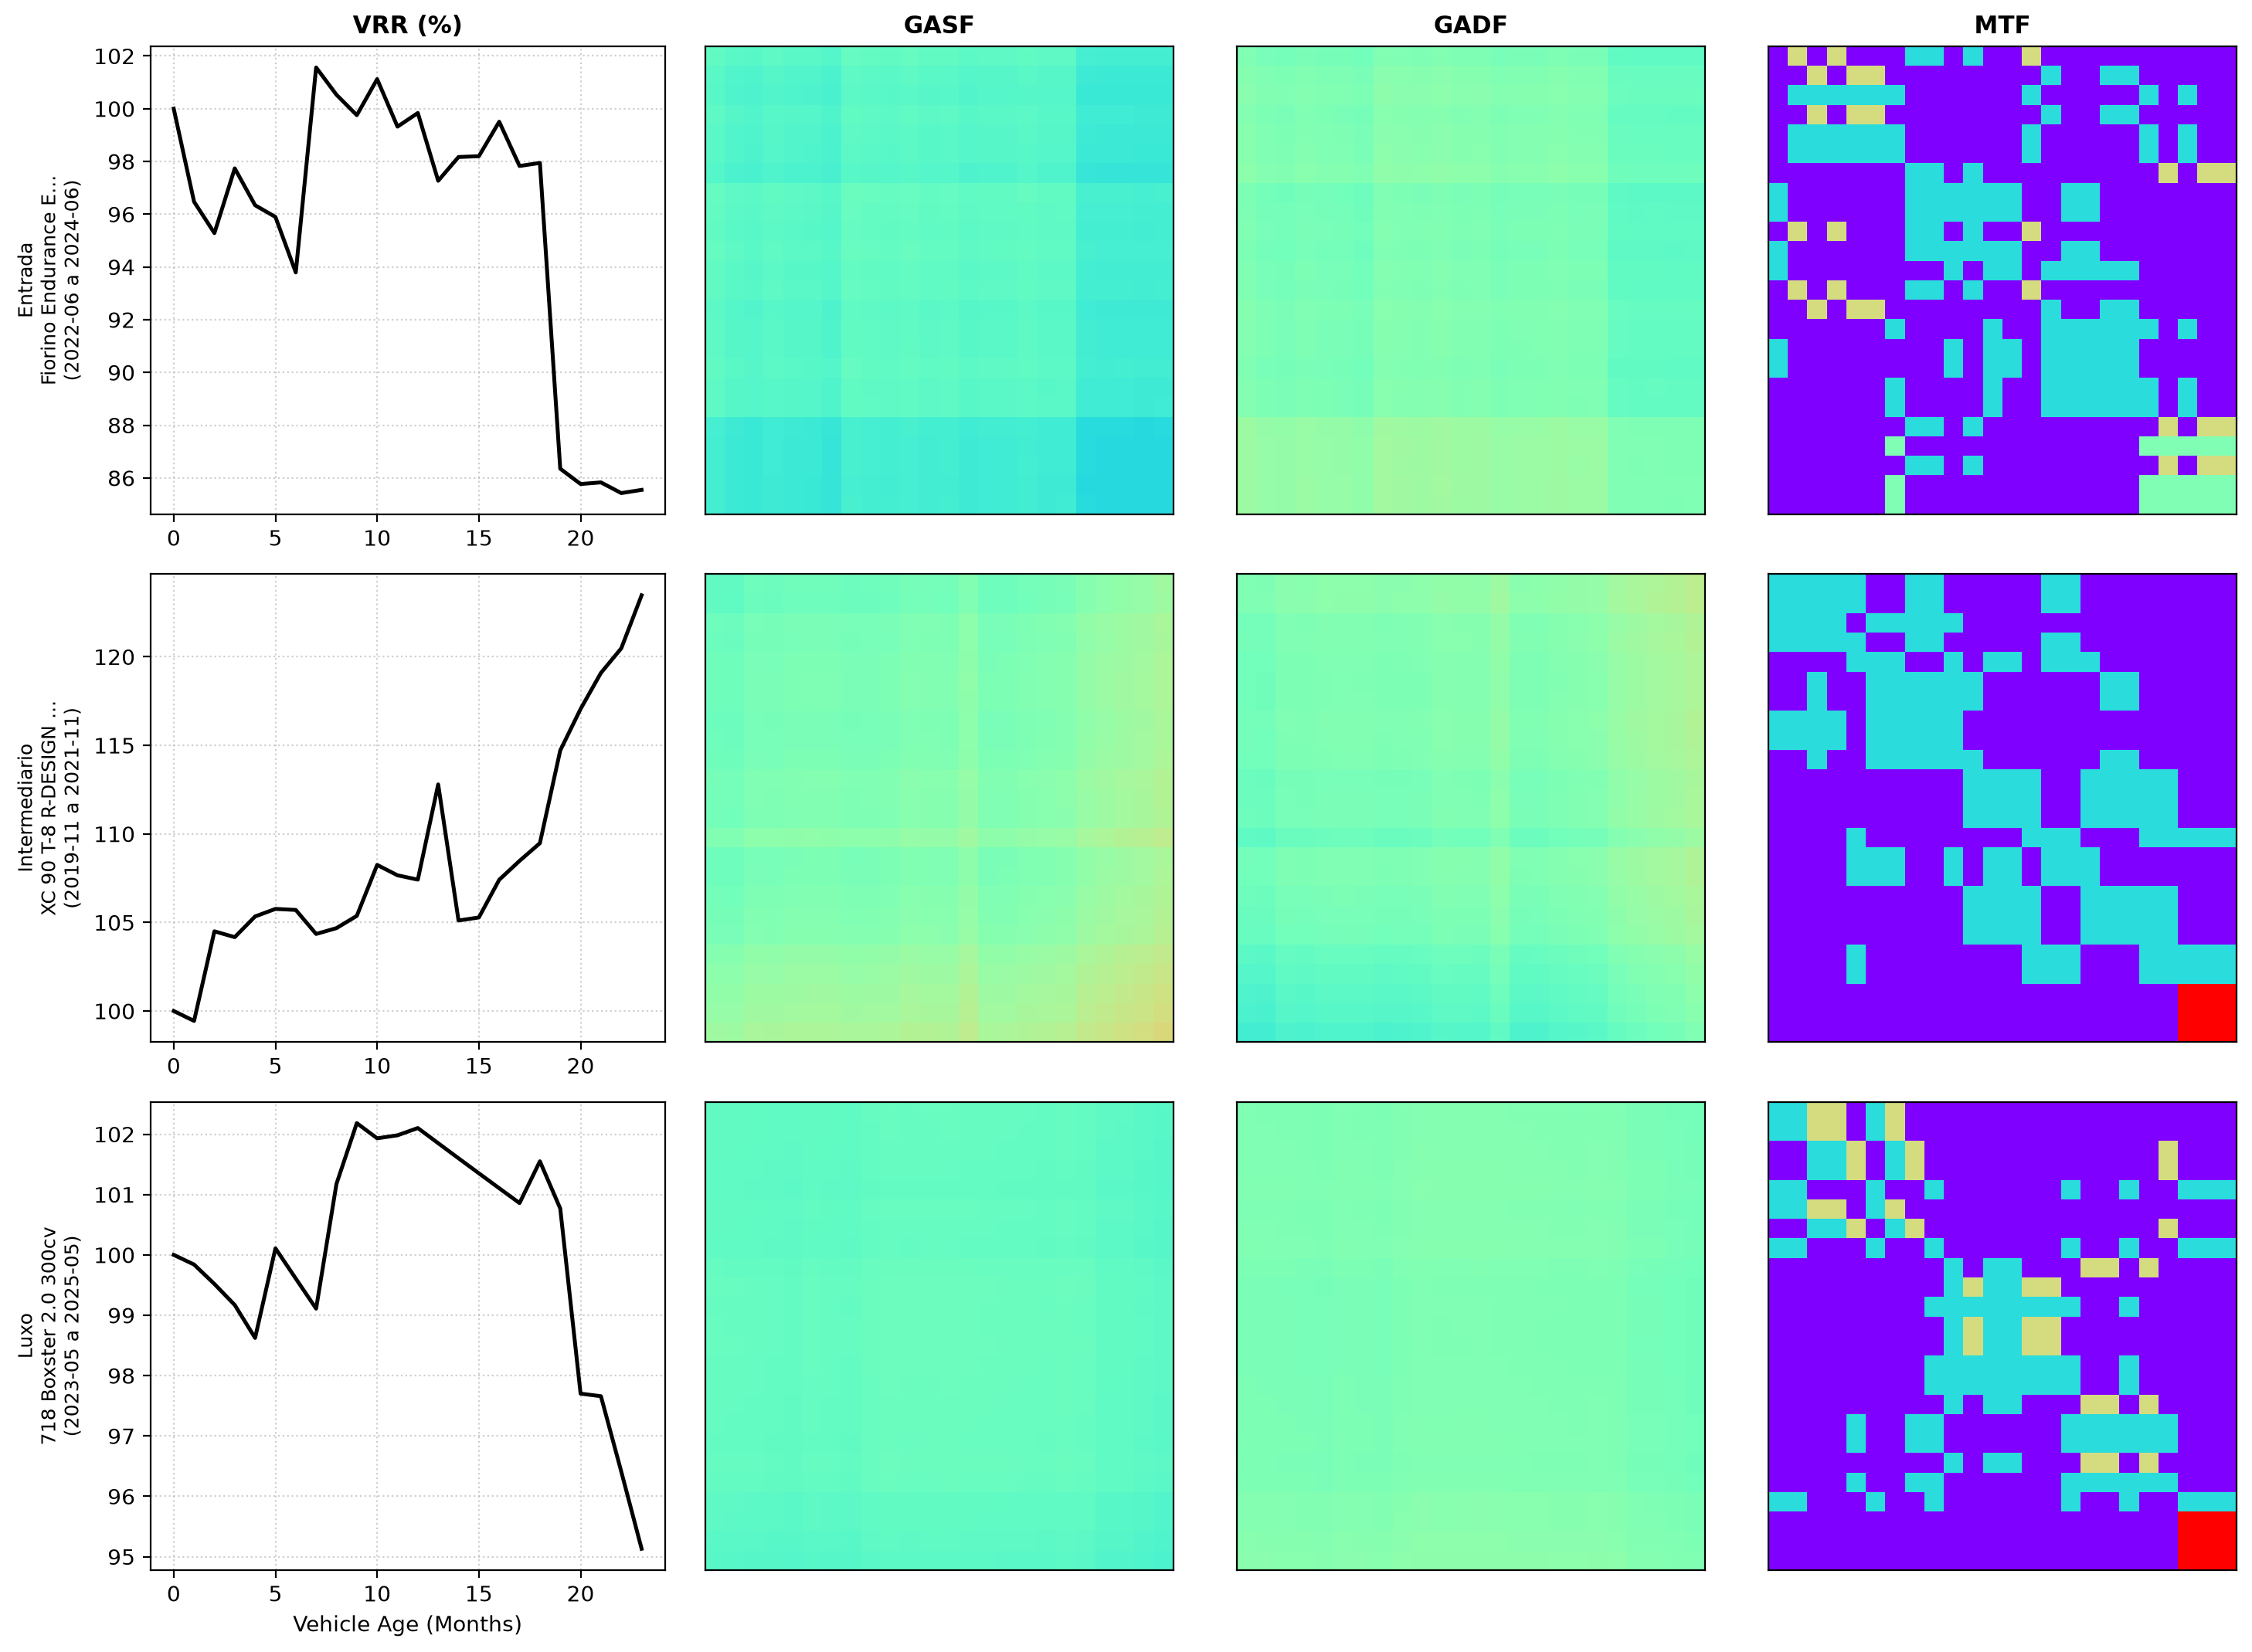
\includegraphics[width=\textwidth]{../../output/encoding/window_24/examples_segments.png}
    \caption{Exemplos por faixa de preço para a janela de 24 meses (imagens $24 \times 24$).}
    \label{fig:w24}
\end{figure}

\begin{figure}[htbp]
    \centering
    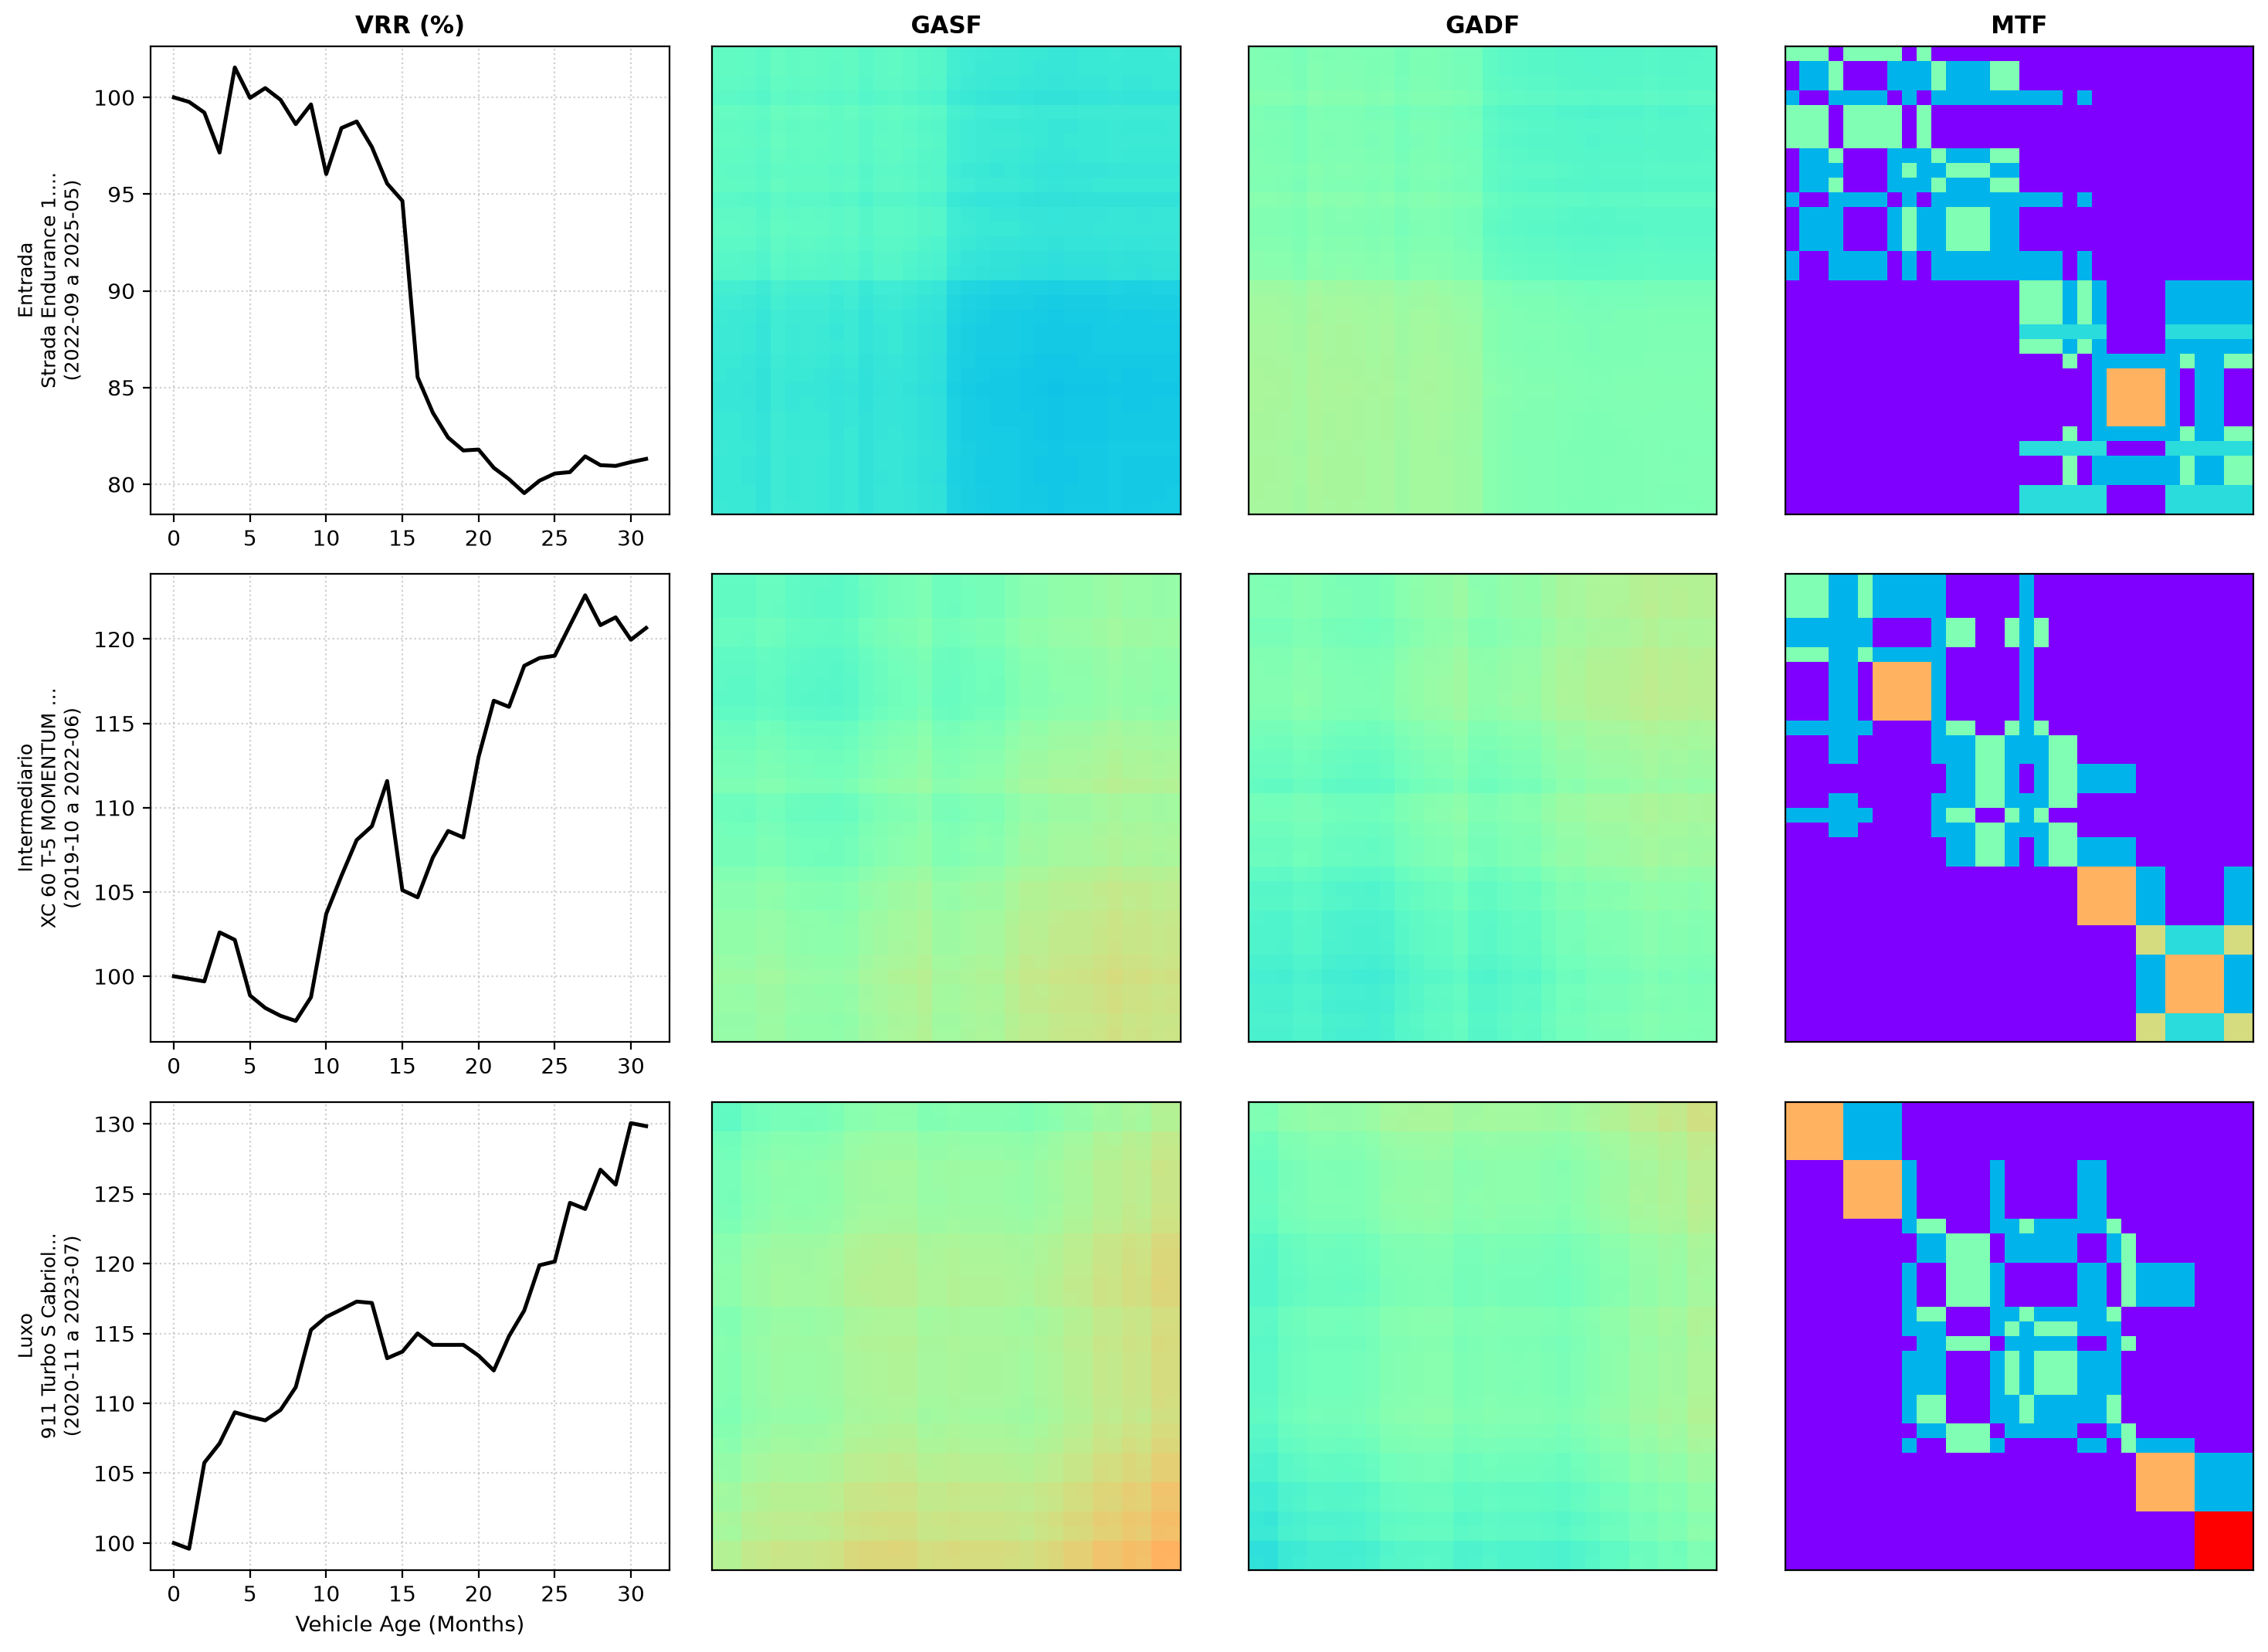
\includegraphics[width=\textwidth]{../../output/encoding/window_32/examples_segments.png}
    \caption{Exemplos por faixa de preço para a janela de 32 meses (imagens $32 \times 32$).}
    \label{fig:w32}
\end{figure}

\begin{figure}[htbp]
    \centering
    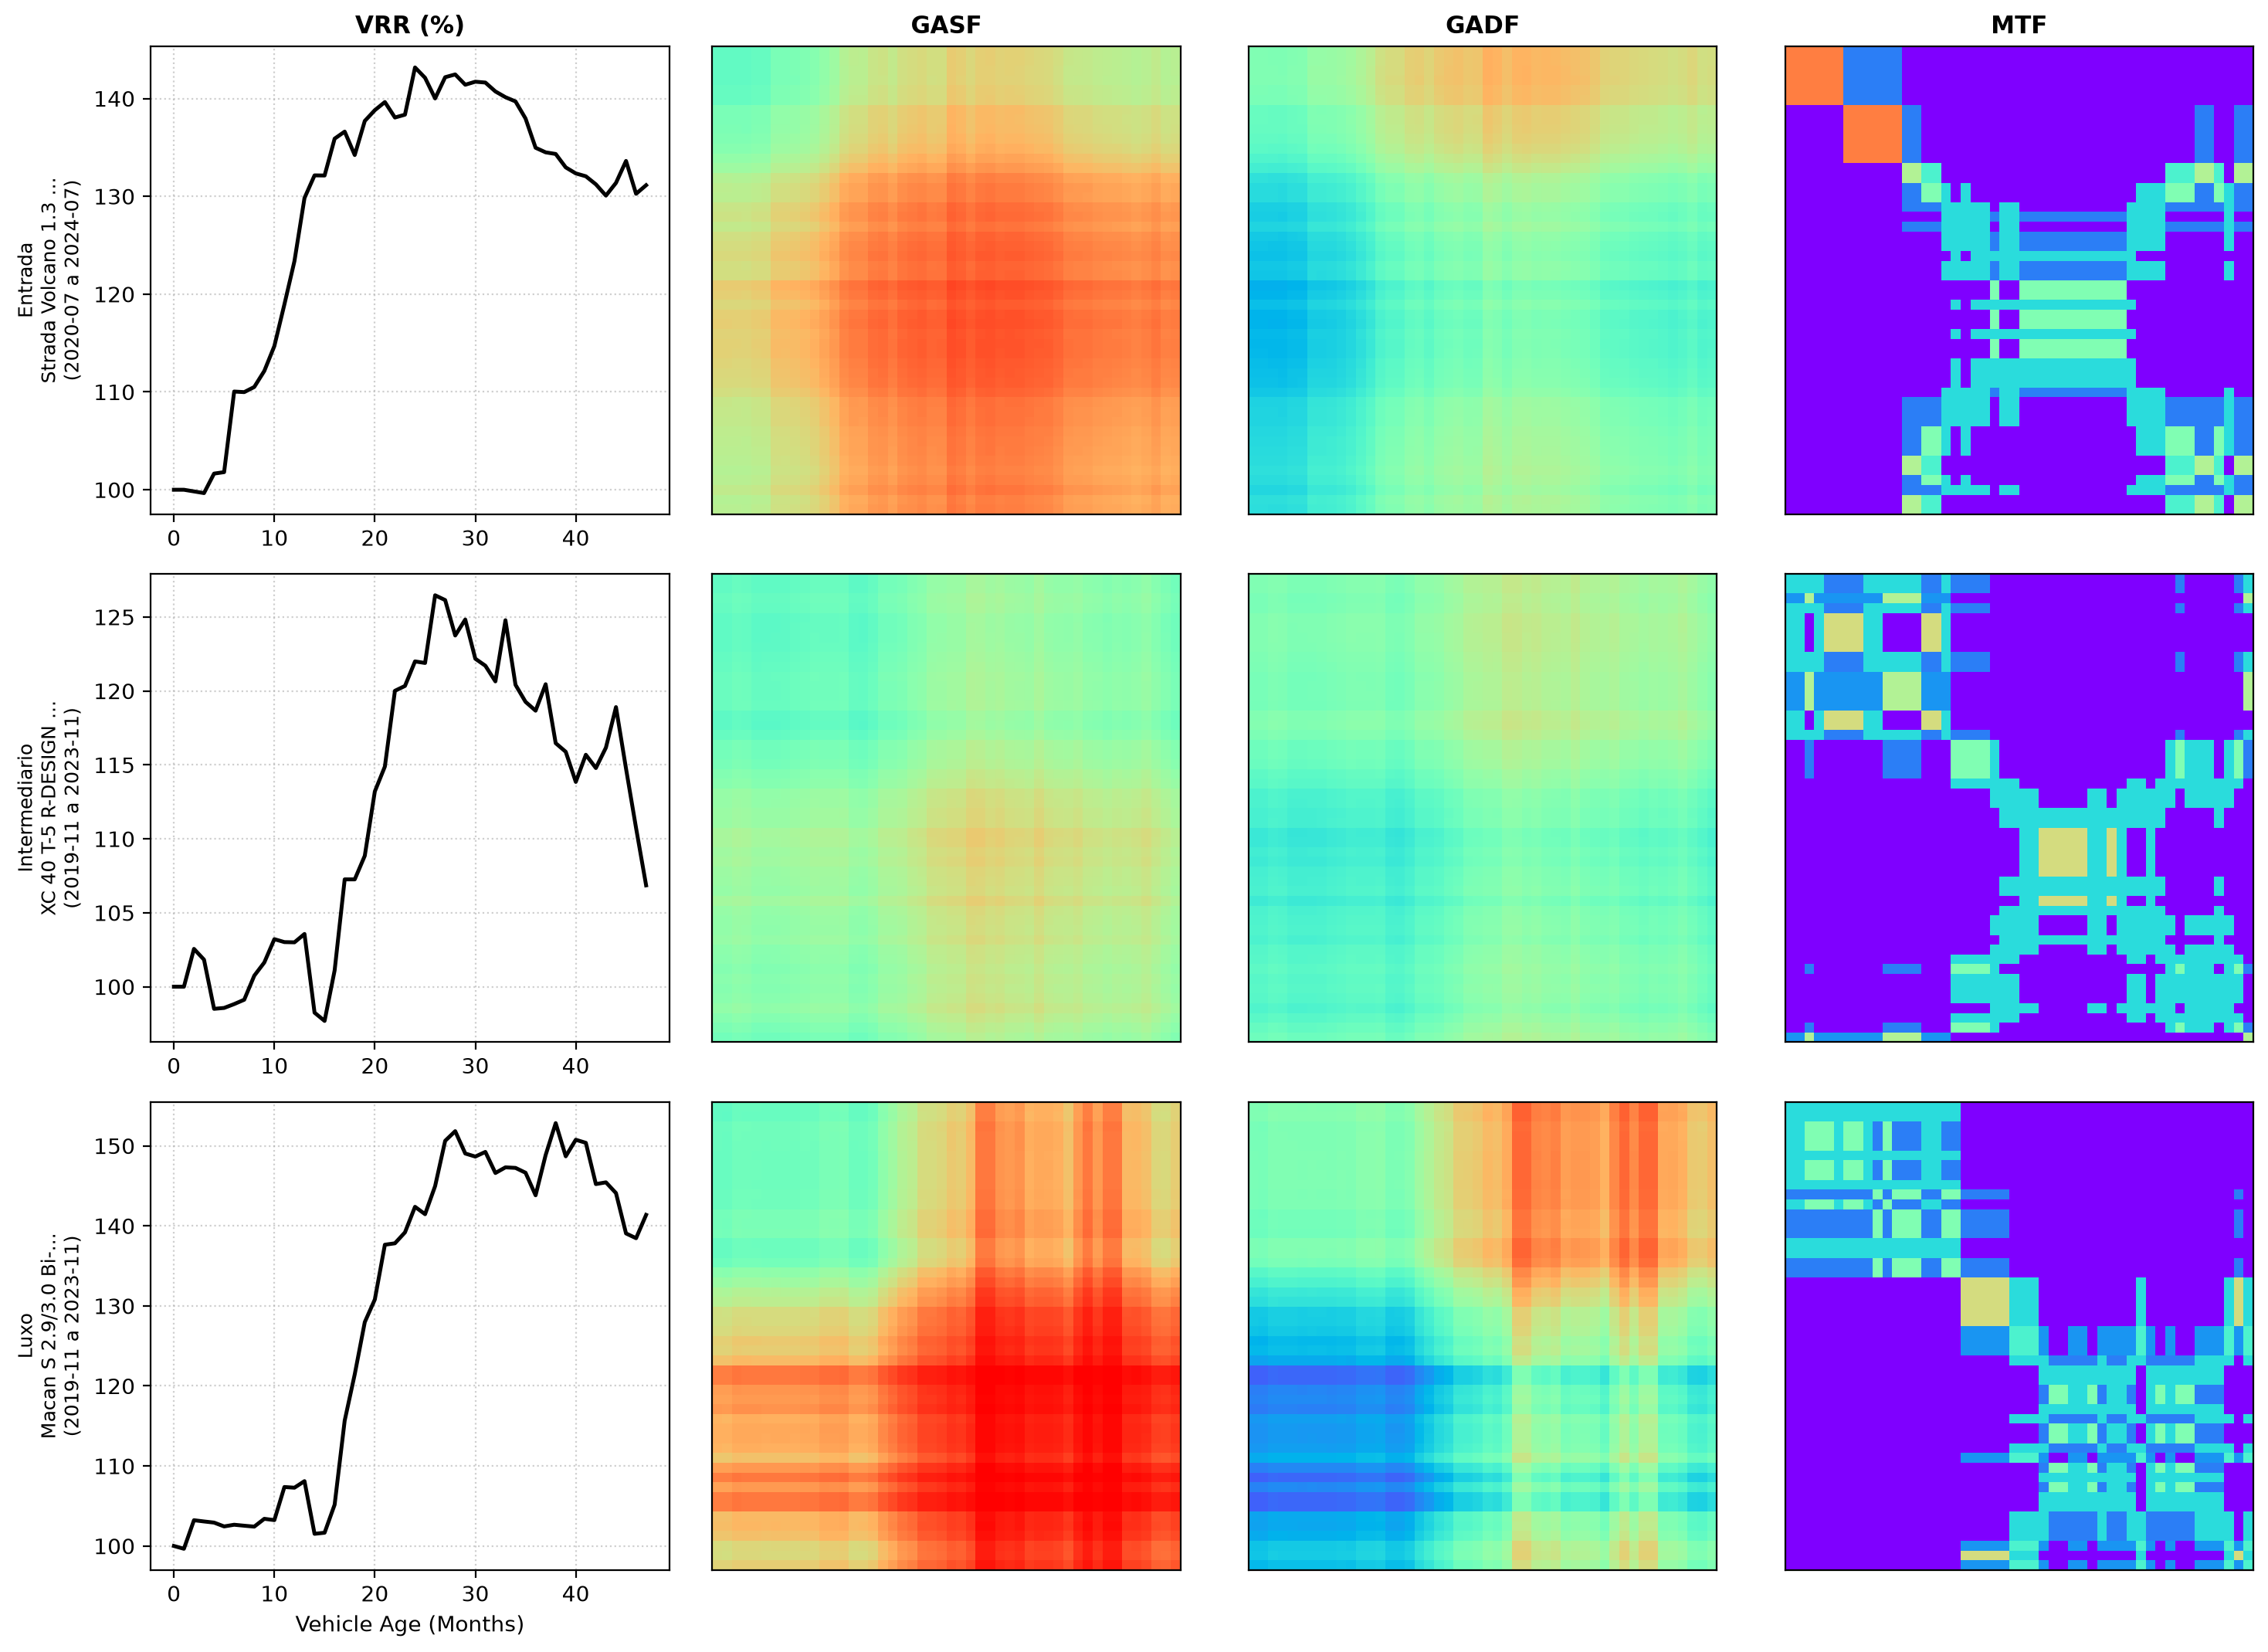
\includegraphics[width=\textwidth]{../../output/encoding/window_48/examples_segments.png}
    \caption{Exemplos por faixa de preço para a janela de 48 meses (imagens $48 \times 48$).}
    \label{fig:w48}
\end{figure}

\begin{figure}[htbp]
    \centering
    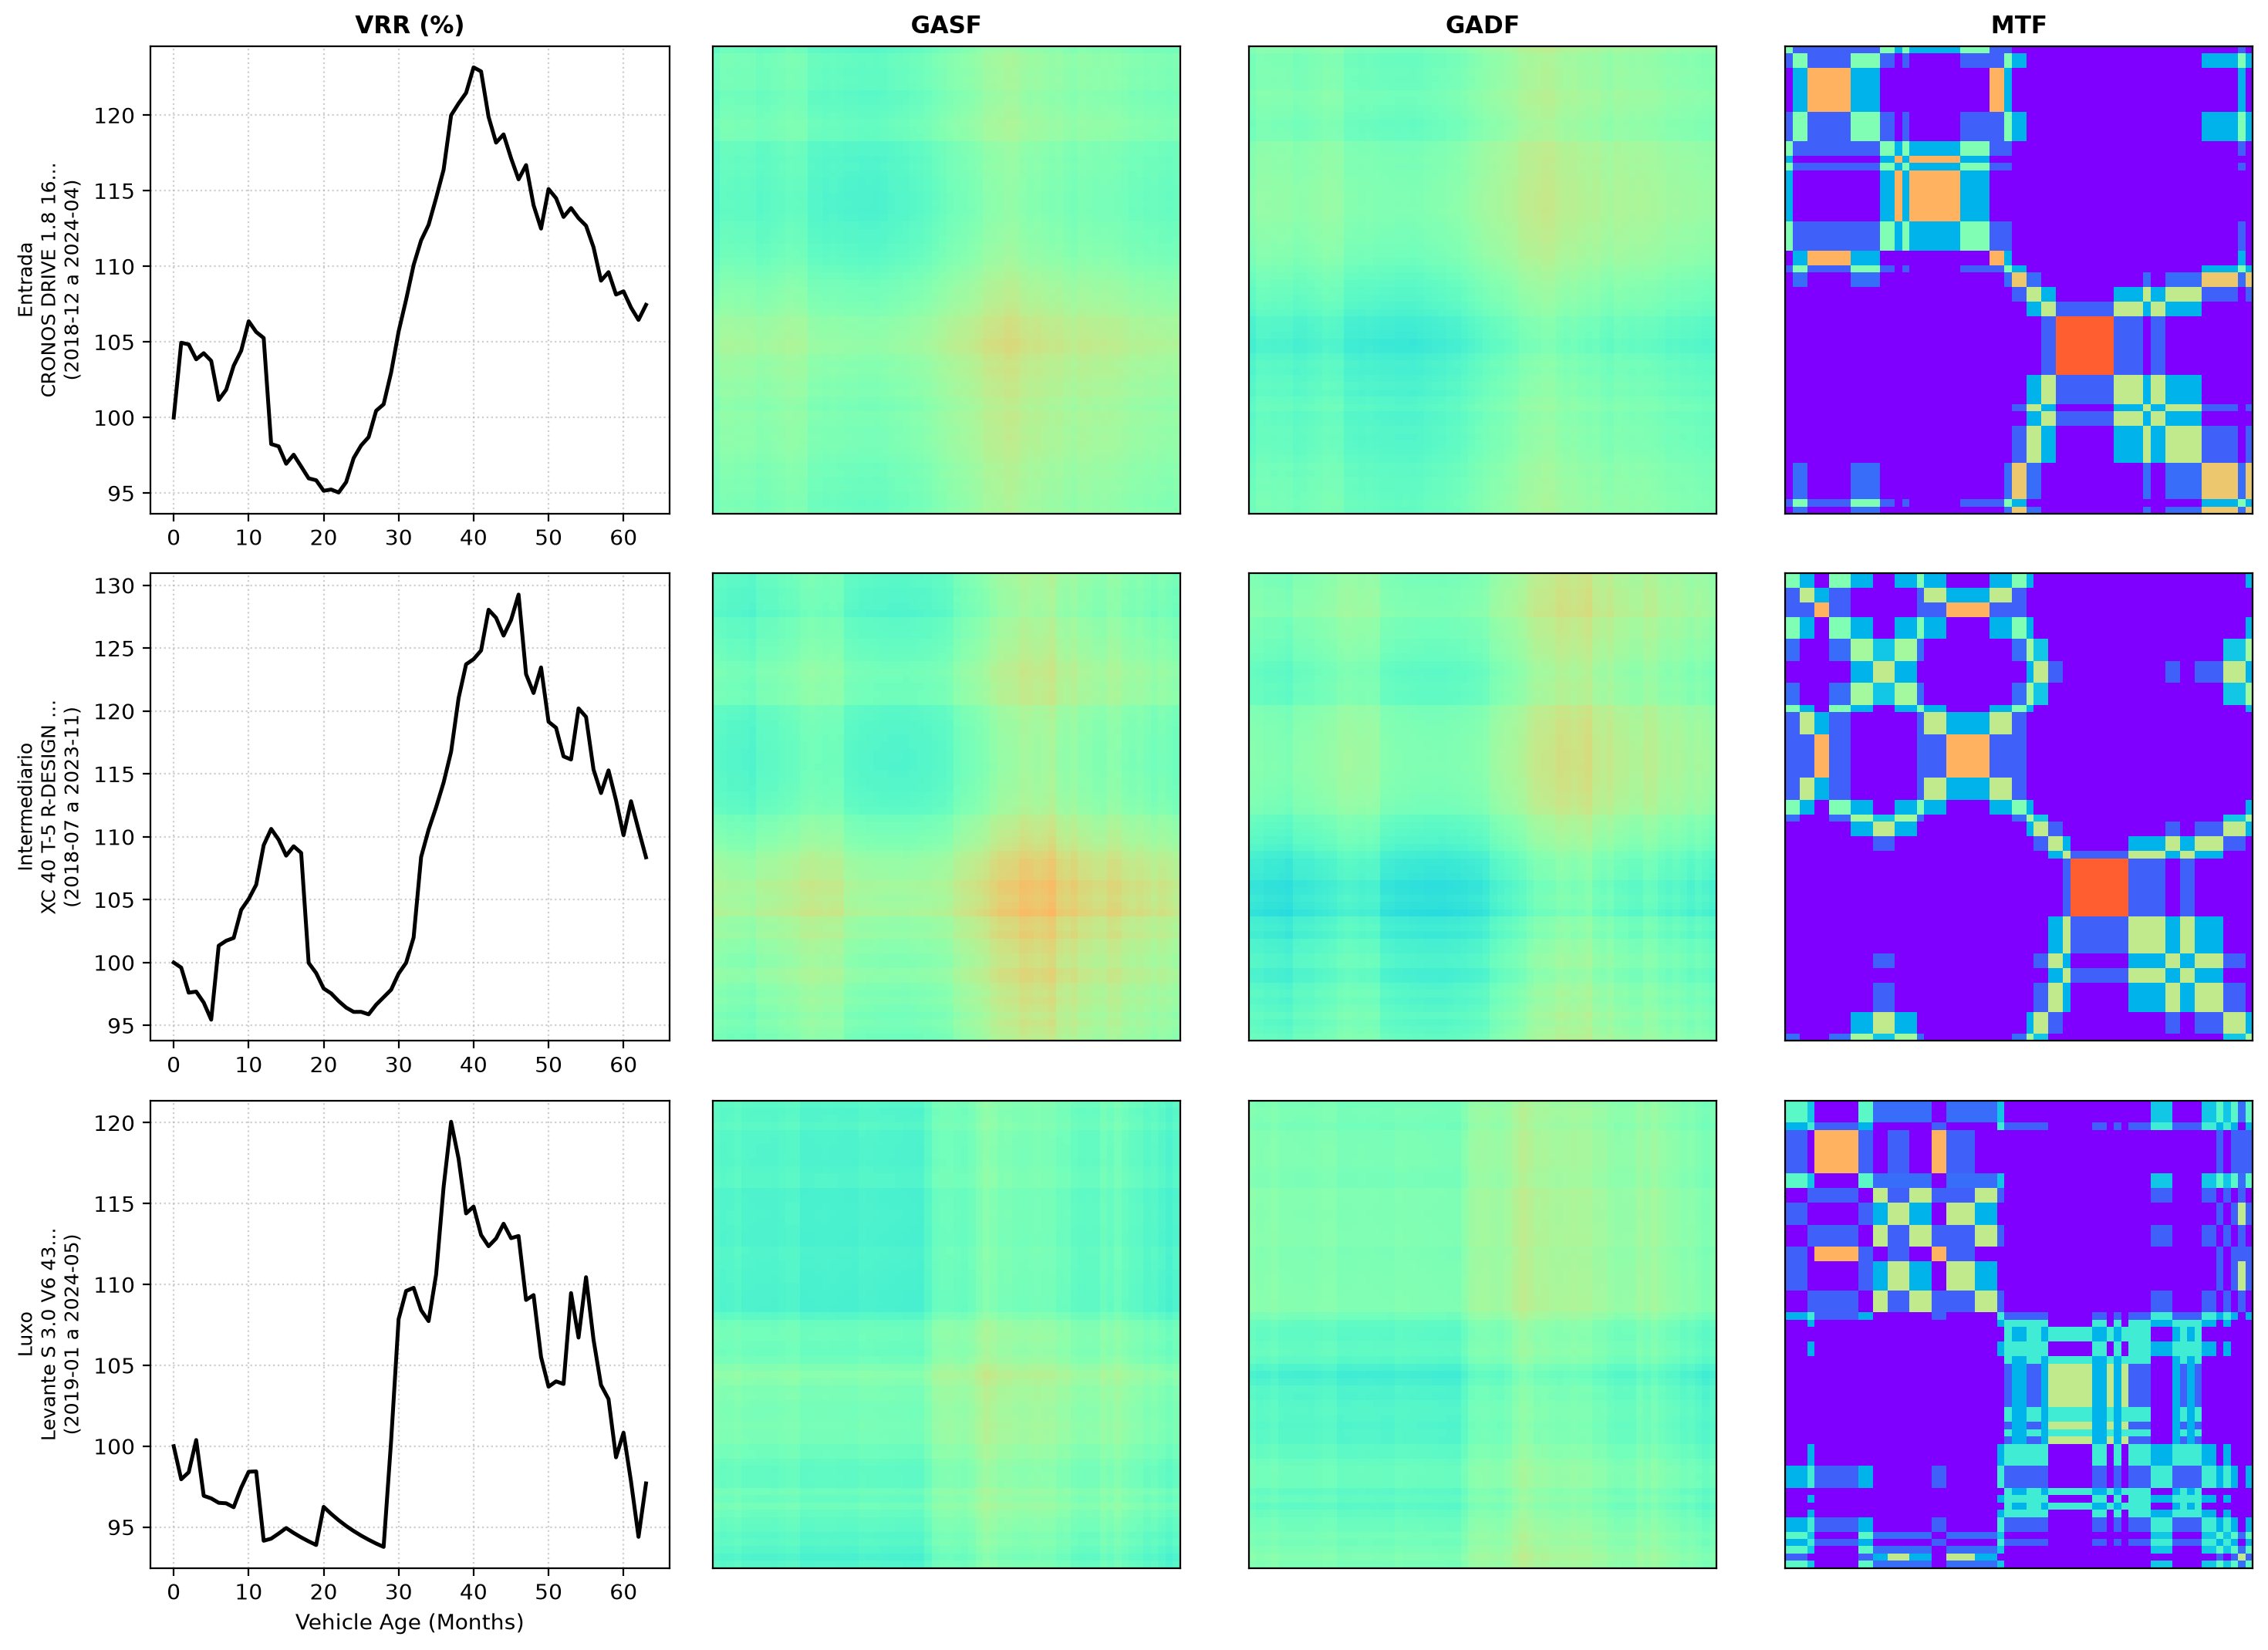
\includegraphics[width=\textwidth]{../../output/encoding/window_64/examples_segments.png}
    \caption{Exemplos por faixa de preço para a janela de 64 meses (imagens $64 \times 64$).}
    \label{fig:w64}
\end{figure}

\subsubsection{Análise das representações}

% \paragraph{GASF e GADF.}
Nos campos angulares, a posição temporal avança do canto superior esquerdo para o inferior direito, e a cor de cada região depende do nível da VRR nos instantes correspondentes, como descrito por \cite{wang2015imaging}. Com a escala global adotada, séries que se afastam muito de $100\%$ geram imagens com contraste forte. É o caso do Macan S na janela de 48 meses (Figura~\ref{fig:w48}), cuja VRR sobe de $100\%$ até cerca de $150\%$ e produz um GASF com grandes regiões em vermelho, e da Strada Volcano na mesma janela, com valorização até cerca de $143\%$. Já séries com pouca amplitude resultam em imagens quase uniformes, como a Fiorino Endurance e o 718 Boxster 2.0 na janela de 24 meses (Figura~\ref{fig:w24}), cuja VRR varia em poucos pontos percentuais. Esse efeito é esperado, pois a escala fixa mantém a informação de nível em vez de normalizar cada série para ocupar todo o intervalo. O GADF, por sua vez, exibe um padrão assimétrico em relação à diagonal (tons azulados e alaranjados em lados opostos), que reflete a diferença de ângulos entre instantes e, portanto, o sentido da variação (subida ou queda) ao longo do tempo. Eventos abruptos aparecem como faixas horizontais e verticais, como a queda de cerca de $98\%$ para $86\%$ no mês 19 da Fiorino (Figura~\ref{fig:w24}) e o salto do Macan S em torno do mês 17 (Figura~\ref{fig:w48}).

% \paragraph{MTF.} 
O MTF apresenta uma estrutura em blocos, em que cada bloco corresponde a um par de quantis e sua probabilidade de transição. Blocos sobre a diagonal e próximos a ela indicam que a série permanece por vários meses no mesmo \textit{bin}, o que é típico de trechos de tendência suave, ao passo que padrões em xadrez e linhas finas indicam alternância mais frequente entre \textit{bins}, ou seja, maior oscilação. Como os quantis são calculados por série, séries com formatos de curva parecidos podem gerar MTF semelhantes mesmo com níveis de VRR diferentes. Isso é consistente com a observação de \cite{wang2015imaging} de que o MTF captura a dinâmica, mas não seria suficiente, sozinho, para reconstruir o sinal. Por essa razão, os autores o tratam como canal complementar aos campos angulares.

% \paragraph{Faixas de preço.}
Nos exemplos, os veículos de Entrada (Toro, Strada, Fiorino) e de Intermediário (Volvo XC40, XC60, XC90, S60) apresentam, em várias janelas, um período inicial de valorização acima do preço de lançamento seguido de queda (Toro e XC60 na janela de 64 meses, XC40 na de 48 meses), enquanto os exemplos de Luxo (Porsche) mostram comportamentos variados: o 911 Turbo S cai para cerca de $86\%$ e se recupera até cerca de $110\%$ na janela de 64 meses, o 718 Boxster S valoriza de forma quase monotônica até cerca de $138\%$ na janela de 32 meses e o Macan S passa de $150\%$ na de 48 meses. A VRR acima de $100\%$ em veículos de 2019 a 2020 sugere que o período observado teve forte valorização do mercado de usados, o que deve ser confirmado na análise exploratória. Como cada faixa é representada por um único veículo por figura, essas observações são qualitativas e não permitem concluir diferenças sistemáticas entre as faixas, o que dependerá das etapas seguintes de classificação ou agrupamento. De qualquer forma, as imagens mostram que trajetórias distintas de depreciação geram texturas visualmente distintas nas três codificações, o que é a premissa para o uso de métodos de visão computacional sobre essas representações, de forma análoga ao que \cite{wu2023imaging} exploram em séries financeiras.

%  \paragraph{Efeito do tamanho da janela.} 
À medida que a janela aumenta, as imagens ganham resolução e passam a conter trechos mais longos da trajetória, incluindo fases de valorização, pico e queda (Figuras~\ref{fig:w48} e \ref{fig:w64}). Nas janelas curtas (24 e 32 meses), as imagens são mais homogêneas e o MTF possui blocos grandes e menos estruturados (Figuras~\ref{fig:w24} e \ref{fig:w32}). Em contrapartida, janelas maiores restringem a amostra aos veículos com histórico mais longo, o que é um compromisso a ser considerado nas etapas seguintes.
